\documentclass[a4paper,14pt]{extreport}
\usepackage[left=1.5cm,right=1.5cm,
    top=1.5cm,bottom=2cm,bindingoffset=0cm]{geometry}
\usepackage{scrextend}
\usepackage[T1,T2A]{fontenc}
\usepackage[utf8]{inputenc}
\usepackage[english,russian,ukrainian]{babel}
\usepackage{tabularx}
\usepackage{amssymb}
\usepackage{color}
\usepackage{amsmath}
\usepackage{mathrsfs}
\usepackage{listings}
\usepackage{graphicx}
\graphicspath{ {./images/} }
\usepackage{lipsum}
\usepackage{xcolor}
\usepackage{hyperref}
\usepackage{tcolorbox}
\usepackage{tikz}
\usepackage[framemethod=TikZ]{mdframed}
\usepackage{wrapfig,boxedminipage,lipsum}
\mdfdefinestyle{MyFrame}{%
linecolor=blue,outerlinewidth=2pt,roundcorner=20pt,innertopmargin=\baselineskip,innerbottommargin=\baselineskip,innerrightmargin=20pt,innerleftmargin=20pt,backgroundcolor=gray!50!white}
 \usepackage{csvsimple}
 \usepackage{supertabular}
\usepackage{pdflscape}
\usepackage{fancyvrb}
%\usepackage{comment}
\definecolor{ggreen}{rgb}{0.4,1,0}
\definecolor{rred}{rgb}{1,0.1,0.1}
\usepackage{array,tabularx}
\usepackage{colortbl}

\usepackage{varwidth}
\tcbuselibrary{skins}
\usepackage{fancybox}




\usepackage{float}
\usepackage{wrapfig}
\usepackage{framed}
%for nice Code{
\lstdefinestyle{customc}{
  belowcaptionskip=1\baselineskip,
  breaklines=true,
  frame=L,
  xleftmargin=\parindent,
  language=C,
  showstringspaces=false,
  basicstyle=\small\ttfamily,
  keywordstyle=\bfseries\color{green!40!black},
  commentstyle=\itshape\color{purple!40!black},
  identifierstyle=\color{blue},
  stringstyle=\color{orange},
}
\lstset{escapechar=@,style=customc}
%}


\begin{document}
\pagecolor{white}
\begin{titlepage}
  \begin{center}
    \large
    Національний технічний університет України \\ "Київський політехнічний інститут імені Ігоря Сікорського"


    Факультет Електроніки

    Кафедра мікроелектроніки
    \vfill

    \textsc{ЗВІТ}\\

    {\Large Про виконання лабораторної роботи №2\\
      з дисципліни: «Алгоритми та структури даних-2»\\[1cm]

        Робота з масивами та списками. Методи сортування та пошуку.


    }

  \bigskip
\end{center}
\vfill

\newlength{\ML}
\settowidth{\ML}{«\underline{\hspace{0.4cm}}» \underline{\hspace{2cm}}}
\hfill
\begin{minipage}{1\textwidth}
Виконавець:\\
Студент 3-го курсу \hspace{4cm} $\underset{\text{(підпис)}}{\underline{\hspace{0.2\textwidth}}}$  \hspace{1cm}А.\,С.~Мнацаканов\\
\vspace{1cm}

Перевірив: \hspace{6.1cm} $\underset{\text{(підпис)}}{\underline{\hspace{0.2\textwidth}}}$  \hspace{1cm}Д.\,Д.~Татарчук\\

\end{minipage}

\vfill

\begin{center}
2020
\end{center}
\end{titlepage}
%--------------------------------1-------------------------------
%\begin{center}\fcolorbox{black}{ggreen}{Варіант № 5}\end{center}
\textbf{Мета роботи} – навчитись використовувати масиви та списки при розробці програм, вивчити методи сортування.\\

\textbf{Завдання}\\
Написати програму, що виконує наступні дії:\\

1) Зчитує дані із файлу отриманого в першій лабораторній роботі та зберігає їх у пам’яті у вигляді структури: \textbf{Список з одинарними зв’язками}.\\

2) Виводить дані на екран у вигляді двох стовпців x   f(x), розділених трьома символами пробілу. Стовпці повинні мати заголовки X та Y відповідно.\\

3) Сортувати дані за зростанням або за спаданням за вибором користувача \textbf{методом виключення}, заданим у таблиці 3 відповідно до варіанту.\\

4) Виводити на екран відсортовану послідовність.\\

5) Здійснювати бінарний пошук введеної з клавіатури величини та виводити на екран результат пошуку. Величини для пошуку (ключі пошуку) повинні зберігатись у програмі у вигляді черги, розмір якої також вводиться з клавіатури. Результати пошуку повинні відображатись на екрані у порядку введення ключів пошуку.\\


\vspace{0.3cm}
\begin{center}\textbf{Виконання роботи}\end{center}
\textbf{Код на С++}\\

\lstinputlisting[language=C++]{Laba-2.cpp}


також тут я написав 2 окремі функції в залежності як ми хочемо відсортувати чиста викликаємо або функцію less, або qwe.

\begin{figure}[h]
\center{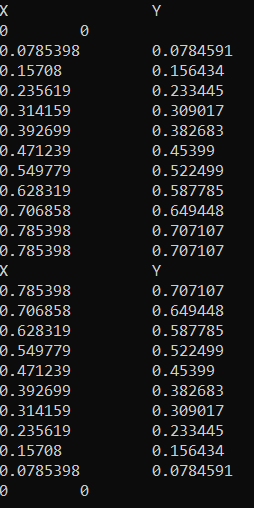
\includegraphics[width=0.4\linewidth]{1.png}}
\caption{Результати.}

\end{figure}














\end{document}
